\documentclass{beamer}
\usepackage[latin9]{inputenc}
\usepackage{xcolor}
\usepackage{graphics, graphicx}
\usepackage{tikz, tkz-graph}
\usepackage{pgf, pgfplots}
\usepackage{graphviz, tkz-berge}
\usepackage{graphics, graphicx}
\usepackage{pstricks, pst-node, pst-tree}
\usepackage{float}

\usetikzlibrary{arrows, petri, topaths}
\usetikzlibrary{shapes}
\usetikzlibrary{arrows.meta}
\usetikzlibrary{positioning,automata}

\usetheme{Warsaw}
\mode<presentation>{\usetheme{Warsaw}}
\setbeamertemplate{caption}{\raggedright\insertcaption\par}

\graphicspath{ {graphics/} }


\title{Els grafs: xarxes, camins i connexions}
 
\subtitle{De la matem�tica discreta a la realitat}
 
\author{Aniol Garcia i Serrano}
 

\date[Presentaci� TDR] % (optional)
{Presentaci� del treball, Gener 2017}



\begin{document}

\begin{frame}{Overview}
\tableofcontents
\end{frame}

\frame{\titlepage}

\section{Introducci�}
\subsection{El meu primer graf}
\begin{frame}
\frametitle{El meu primer graf}
	\begin{figure}[H]
		\includegraphics[scale=0.3]{graf1}
	\end{figure}
\end{frame}

\subsection{El primer graf}
\begin{frame}
\frametitle{El primer graf}
\begin{columns}
 
\column{0.5\textwidth}
\begin{figure}[H]
\centering
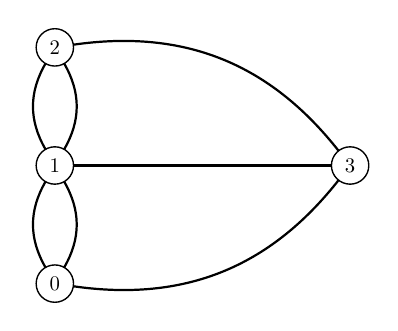
\begin{tikzpicture}[scale=0.75,transform shape]
  \Vertex[x=0,y=0]0
  \Vertex[x=0,y=2]1
  \Vertex[x=0,y=4]2
  \Vertex[x=5,y=2]3
  \tikzstyle{LabelStyle}=[fill=white,sloped]
  \Edge(1)(3)
  \tikzstyle{EdgeStyle}=[bend left]
  \Edge(0)(1)
  \Edge(1)(2)
  \Edge(2)(3)
  \tikzstyle{EdgeStyle}=[bend right]
  \Edge(0)(1)
  \Edge(1)(2)
  \Edge(0)(3)
\end{tikzpicture}
\end{figure}

\pause

\column{0.5\textwidth}
\includegraphics[scale=0.5]{Konigsberg_bridges}

\end{columns}
\end{frame}

\subsection{Breu hist�ria}
\begin{frame}
\frametitle{Breu hist�ria}
\begin{columns}
 
\column{0.5\textwidth}
	\begin{figure}[H]
		\includegraphics[scale=0.21405]{Euler}
		\caption{Leonhard Euler}
	\end{figure}
\column{0.5\textwidth}
	\begin{figure}[H]
		\includegraphics[scale=0.4]{Leibniz}
		\caption{Gottfried W. Leibniz}
	\end{figure}
\end{columns}
\end{frame}

\frame{\titlepage}


\section{Organitzaci�}
\begin{frame}
\tableofcontents
No hi ha d'haver aquest �ndex, sin� el del treball (simplificat, evidentment)
\end{frame}


\subsection{Tipus de grafs}
\begin{frame}
\begin{columns}
\column{0.5\textwidth}
	\begin{figure}[H]
		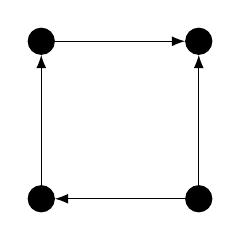
\begin{tikzpicture}[round/.style={circle, draw=black, fill=black, thin, minimum size=1mm}, transform shape]
			\node[round] (a) at (0,0){};
			\node[round] (b) at (0,2) {};
			\node[round] (c) at (2,0) {};
			\node[round] (d) at (2,2) {};
			\draw (a) edge[->, -Latex] (b);
			\draw (c) edge[->, -Latex] (a);
			\draw (b) edge[->, -Latex] (d);
			\draw (c) edge[->, -Latex] (d);
		\end{tikzpicture}
		\caption{Graf dirigit}
	\end{figure}
\column{0.5\textwidth}
\begin{figure}[H]
		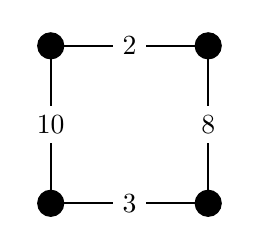
\begin{tikzpicture}[round/.style={circle, draw=black, fill=black, thin, minimum size=1mm}, transform shape]
			\node[round] (a) at (0,0){};
			\node[round] (b) at (0,2) {};
			\node[round] (c) at (2,0) {};
			\node[round] (d) at (2,2) {};
			\Edge[label=$10$](a)(b)
			\Edge[label=$3$](c)(a)
			\Edge[label=$2$](b)(d)
			\Edge[label=$8$](c)(d)
		\end{tikzpicture}
		\caption{Graf ponderat}
	\end{figure}

\end{columns}
\end{frame}

\begin{frame}
\begin{figure}[H]
		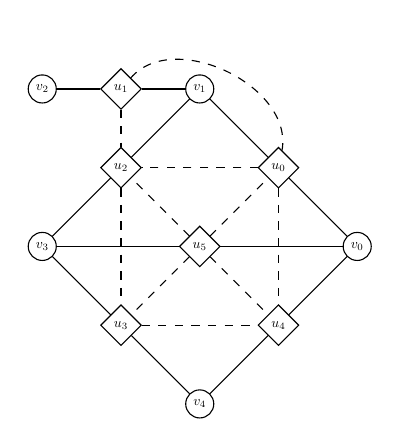
\begin{tikzpicture}[round/.style={circle, draw=black, thin, minimum size=.5mm}, transform shape, scale=0.5]
			\node[round] (a) at (8,4){$v_{0}$};
			\node[round] (b) at (4,8){$v_{1}$};
			\node[round] (c) at (0,8){$v_{2}$};
			\node[round] (d) at (0,4){$v_{3}$};
			\node[round] (e) at (4,0){$v_{4}$};
			\node[draw, diamond] (f) at (6,6){$u_{0}$};
			\node[draw, diamond] (g) at (2,8){$u_{1}$};
			\node[draw, diamond] (h) at (2,6){$u_{2}$};
			\node[draw, diamond] (i) at (2,2){$u_{3}$};
			\node[draw, diamond] (j) at (6,2){$u_{4}$};
			\node[draw, diamond] (k) at (4,4){$u_{5}$};
			\draw (a) edge (f);
			\draw (a) edge (j);
			\draw (a) edge (k);
			\draw (f) edge (b);
			\draw (j) edge (e);
			\draw (k) edge (d);
			\draw (b) edge (g);
			\draw (g) edge (c);
			\draw (b) edge (h);
			\draw (h) edge (d);
			\draw (d) edge (i);
			\draw (i) edge (e);
			
			\draw (f) edge[dashed] (h);
			\draw (k) edge[dashed] (f);
			\draw (k) edge[dashed] (j);
			\draw (k) edge[dashed] (i);
			\draw (k) edge[dashed] (h);
			\draw (f) edge[dashed] (h);
			\draw (i) edge[dashed] (j);
			\draw (g) edge[dashed] (h);
			\draw (f) edge[dashed] (j);
			\draw (h) edge[dashed] (i);
			\draw (g) edge[dashed, bend left=75] (f);
			
		\end{tikzpicture}	
\end{figure}
\caption{Graf Lineal}
\end{frame}


\begin{frame}
\begin{enumerate}
\item<1-| alert@1> Suppose $p$ were the largest prime number.
\item<2-> Let $q$ be the product of the first $p$ numbers.
\item<3-> Then $q+1$ is not divisible by any of them.
\item<1-> But $q + 1$ is greater than $1$, thus divisible by some prime
number not in the first $p$ numbers.\qedhere
\end{enumerate}
\end{frame}

\end{document}